% SISC 3 : Software and High-Performance Computing. Papers in this category should concern the novel design and development of computational methods and high-quality software, parallel algorithms, high-performance computing issues, new architectures, data analysis, or visualization. The primary focus should be on computational methods that have potentially large impact for an important class of scientific or engineering problems.

\documentclass[review]{siamart1116}

\newcommand{\blue}[1]{\textcolor{blue}{[#1]}}
\newcommand{\red}[1]{\textcolor{red}{[#1]}}
\newcommand{\green}[1]{\textcolor{green}{[#1]}}

\begin{document}

\title{The Adaptive Multiscale Simulation Infrastructure - Methods and Soft-tissue Example Simulation}

% Authors: full names plus addresses.
\author{
  William R. Tobin \thanks{Scientific Computational Research Center, Rensselaer Polytechnic Institute, Low Center for Industrial Innovation, CII-4011, 110 8th Street, Troy, NY 12180.} 
  \and
  Victor W.L. Chan\footnotemark[1]
  \and
  Catalin R. Picu\footnotemark[1] \thanks{Department of Mechanical, Aerospace and Nuclear Engineering, Rensselaer Polytechnic Institute, Jonsson Engineering Center, Rm.\ 2049, 110 8th Street, Troy, NY 12180.}
  \and
  Victor H. Barocas\thanks{Department of Biomedical Engineering, University of Minnesota, 7-105 Nils Hasselmo Hall, 312 Church Street SE, Minneapolis, MN 55455.}
  \and
  Mark S. Shephard\footnotemark[1].
}
\date{\today}
\maketitle

\begin{abstract}
\red{Discuss multi-scale and frameworks, show how AMSI does multi-scale, and how it is different than others. Introduce the soft-tissue problem. Discuss hierarchical multi-scale and relate it to well-known multi-scale models, and what requirements it imposes. Discuss AMSI design decisions, the implementation of AMSI, and how to use AMSI to implement the soft tissue simulation. Show some performance measures relevant to the implementation of this sort of simulation, and finally produce a roadmap on how to apply AMSI to other simulations (hierarchical and concurrent).}

\end{abstract}

\section{Introduction}\label{sec:intro}

\subsection{Multi-scale Simulation}\label{sec:multiscale}

The development of new numerical simulations has proliferated rapidly in the last several decades. The massive increases in computational power of massively parallel machines has facilitated the implementation and execution of numerical simulations of unprecedented scale and fidelity. However, when it is the case that the governing physical mechanism of interest in a simulation occurs at a scale orders removed from the desired resolution of the solution, even the massive increases in computational power of the last decades is insufficient in many cases. Multi-scale simulation techniques offer a method of achieving accurate results on a domain orders of magnitude removed from the underlying phenomena guiding the physical action of the simulation.

Multi-scale simulation broadly falls into two categories: concurrent (partitioned-domain) and hierarchical problems. These categories are most readily distinguished by the relationships between the interacting scales in a problem.

In concurrent problems the domain of each scale is modeled using similar physical dimensions: the standard units used to describe the scale will typically fall within several orders of magnitude of each other. Interface surfaces or regions between the scale domains are used to transfer relevant physical tensor field information between scales. The transfer of relevant tensor field values allow the scales to influence one another and gives rise to multi-scale behaviors in the problem simulation. Often values in concurrent simulations will not require the use of up- or down-scaling operations to transfer tensor values. 

The Domain Decomposition Methods (DDM) \cite{toselli2005domain} and the Quasicontinuum Methods (QM) \cite{miller2002quasicontinuum} both allow the implementation of concurrent multi-scale problems. DDM allows the implementation of multi-physics continuum-to-continuum coupling while QM is used to couple atomistic models to continuum regions in a macro-scale domain.

%Most continuum/continuum coupling problems fall into this category when the scale separation is sufficiently small. This class of problem also includes atomistic/continuum couplings \cite{miller2009unified}, in which the scales may often be separated by more than several orders of magnitude.

Hierarchical problems are characterized by strongly-separated scales in which the physical dimensions of the scale are typically 6 or more orders of magnitude separated. The domain relationship between two such scales is often reduced to the existence of micro-scale simulations occurring at various points throughout the larger-scale simulation. The tensor field couplings which give rise to multi-scale behavior occur at each point in the macro-scale simulation at which a micro-scale simulation is embedded. The local value of tensor field data is used to establish conditions at the micro-scale, which in turn produces a tensor field value relevant to the evolution of the macro-scale simulation. Values in hierarchical simulations are more likely to require up- and down-scaling operations to account for  differences between the coupled scales.

Hierarchical problems can be implemented with the use of information passing schemes in which a well-defined set of parameters is transmitted between the simulation scales \cite{weinan2011principles,buehler2006concurrent,fish2010multiscale}. This approach allows the replacement of a constitutive model commonly used in continuum mechanics problems with a full single-scale simulation conducted at a distinct points in the macro-scale problem.

The Heterogeneous Multiscale Methods (HMM) \cite{weinan2003heterogenous,weinan2007heterogeneous} are methods used to solve multi-scale problems with either localized regions of macroscopic model failure or problems without a known macroscopic model entirely. HMM is well-suited for application to hierarchical problems as it does not require the existence of a macro-scale constitutive model, allowing the micro-scale simulations to fully guide system behavior.

%The Soft Biological Tissue problem discussed in section \ref{sec:bio-implementation} is an instance of this case of an HMM problem.
%Continuum/continuum problems with strongly-separated scales fall into the hierarchical category,

An example of scale separation maps \cite{borgdorff2013foundations} associated with these multi-scale problem categories can be seen in figure \ref{fig:scale-map}. Further discussion of the taxonomy of multi-scale modeling in \cite{tadmor2011modeling} is a useful primer on the various categories of multi-scale models, with accompanying examples for each category to further elucidate the concepts. 

\begin{figure}
  \centering
  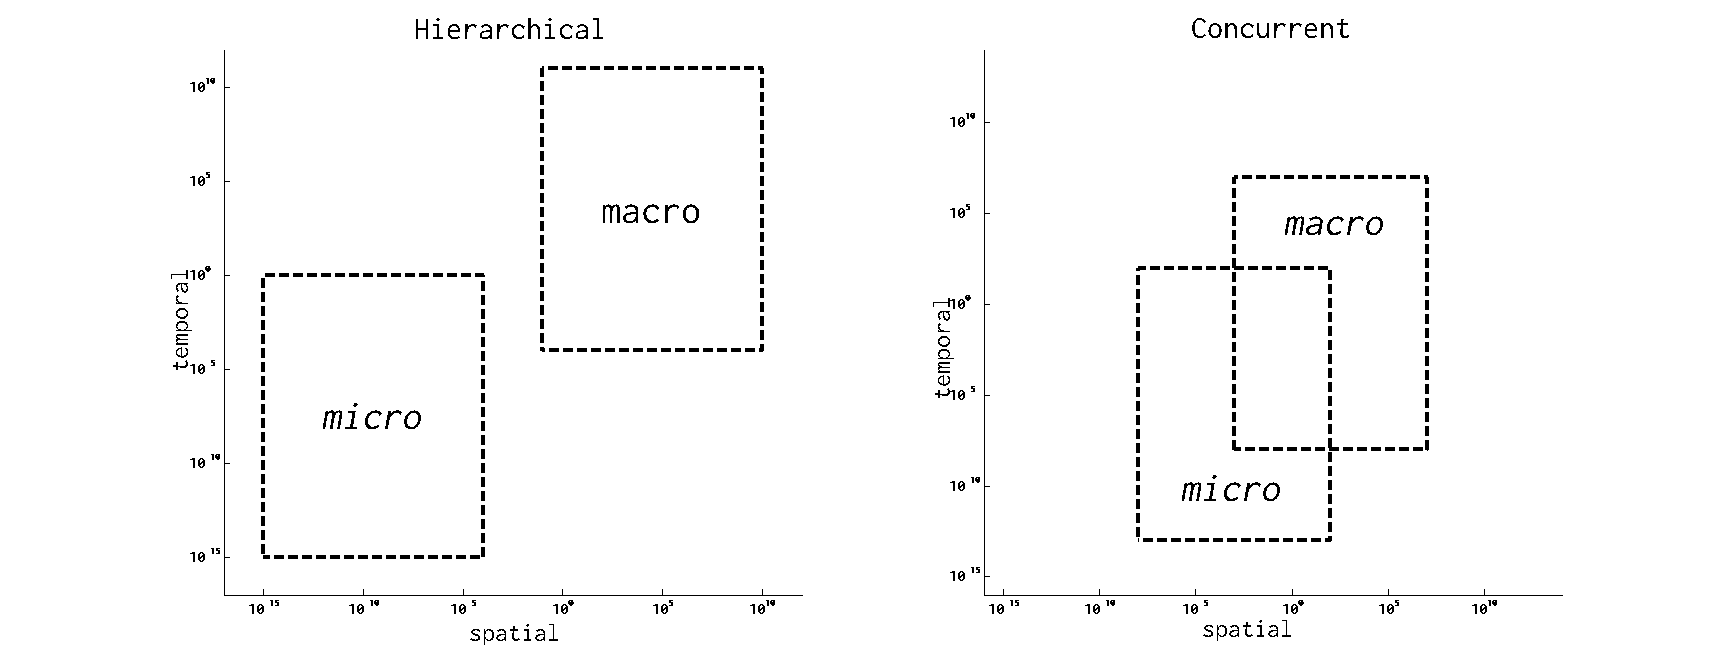
\includegraphics[width=.9\columnwidth]{scale-separation-map}
  \caption{Scale separation maps for hierarchical and concurrent multi-scale problems, respectively.}
  \label{fig:scale-map}
\end{figure}

In the rest of this paper we will discuss currently existing multi-scale frameworks including particulars of their implementations and use cases. We will then discuss the Adaptive Multi-scale Simulation Infrastructure (AMSI) tools we have developed including our intent in development and targeted problem types, the design of our system, and the subsequent implementation of that design. We will further discuss the application of our infrastructure to the development of a multi-scale soft biological tissue simulation. We then discuss the performance of the soft tissue simulation and how this relates to the AMSI multi-scale coupling approach. Finally we will discuss our plans for future development and extension of the capabilities of our infrastructure.

\section{Multi-scale Frameworks}\label{sec:frameworks}

There are numerous multi-scale frameworks currently in development intended to facilitate the implementation of multi-scale simulations on HPC machines. We do not intend to provide a full survey of such frameworks in this section but rather to discuss several frameworks which exhibit features common to many frameworks existing in the multi-scale space at this moment.

Software intended to support multi-scale simulations needs to ”enable the introduction of new models, algorithms, and data structures \cite{keyes2013multiphysics}. Further, a set of well-defined modules with distinct interfaces must be implemented, especially as this concerns data ownership and simulation state. State data must be query-able through interfaces in order for coupled codes to maintain consistency throughout the simulation. Further, implementing general code, or providing mechanisms to extract important underlying data in general formats is necessary. This forces multi-scale application developers to adhere to specific data structures and algorithms, or write their own wrapper code in order to translate specialized data structures into more general formats. These issues and rationales for multi-scale software development are further discussed in\cite{keyes2013multiphysics}.

The Uintah Problem Solving Environment (PSE) \cite{berzins2010uintah} is a framework developed at the University of Utah intended to allow the intuitive combination of parallel simulation components into novel scientific applications, including but not limited to multi-scale simulations. Each component in the Uintah system is designed to solve a PDE on a structured AMR grid, and must adhere to a C++ API used to establish connections between components. All components are decomposed into a set of discrete tasks, each of which has a well-defined set of required input and output data. The information about these tasks is expressed in the form of a directed acyclic graph (DAG) \cite{berzins2015extending}, and is used by the Uintah system to schedule task execution across the HPC system. The parallel communication necessary to provide task input and output occurs through a data warehousing structure which controls access to local and global data.

The Mesh-Based Parallel Code Coupling Interface (MpCCI) \cite{joppich2006mpcci} is a library which facilitates the coupling of simulation codes based on the underlying domain grid over which simulation data (specifically tensor field values) are distributed. Support for different grid formats is provided by MpCCI, as well as different methods of data interpolation when needed to communicate data between simulation scales with mismatched grids. MpCCI uses a code-coupler component object in order for two single-scale application codes to communicate with eachother \cite{delalondre2010collaborative}. A coupler object is implemented to transform values from a producing single-scale code into values that can be used by a consuming single-scale code.

In the time since MpCCI was developed over a decade ago it has seen sufficent adoption to warrant the organization of several user forums and is currently used to support the implementation of multi-physics codes. There have also been coupler objects implemented to allow many industry-standard simulation tools to be coupled through MpCCI including Abaqus, ANSYS Fluent, MATLAB, and others \cite{mpcci-website}.

The \verb=MUSCLE-HPC= \cite{belgacem2017muscle} code is a partial implementation of the \verb=MUSCLE-2= toolkit \cite{borgdorff2014distributed} for use on HPC machines. The multi-scale simulation in \verb=MUSCLE-HPC= is constructed from a set of submodels, each of which is implemented by inheriting from an abstract C++ class which provides an API for initialization, boundary condition updates, numerical solution iteration, and several data query functions. Coupling together of submodels into a multi-scale model is done through the use of an interface of Conduits which the class API has methods to express the set of input and output Conduits for the submodel. Further the \verb=MUSCLE-HPC= runtime environment requires that a machine core acting as a server is devoted to running a special Manager class to register client submodels and facilitate the creation of parallel communication channels between the submodels. 



%\red{there should be some technical depth on each of the frameworks, a clear indication of the goals of the system design and summary of capabilities}

%\subsection{Multi-scale Methods}\label{sec:multi-scale-methods}
%\red{Dig a little deeper into multi-scale, discuss the computational aspects of this type of multi-scale, and reference some well-known multi-scale models that fall into this category.}

%As noted in section \ref{sec:multiscale}, hierarchical multi-scale problems are characterized by the strongly-separated nature of the single-scale components interacting in the problem. This allows the scales to be coupled with minimal-to-no inter-domain introspection operations. Thus these problems can be implemented with the use of information passing schemes in which a well-defined set of parameters is transmitted between the simulation scales \cite{weinan2011principles,buehler2006concurrent,fish2010multiscale}. This approach allows the replacement of a constitutive model commonly used in continuum mechanics problems with a full single-scale simulation conducted at a distinct points in the macro-scale problem.

%The Heterogeneous Multiscale Methods (HMM) \cite{weinan2003heterogenous,weinan2007heterogeneous} is a model used to solve multi-scale problems with either localized regions of macroscopic model failure or problems without a known macroscopic model entirely. The HMM has a microscopic process acting on physical field \verb-u- and a macroscopic process acting on field \verb+U+, defined over domains \verb-d- and \verb+D+ respectively. The physical processes at each scale acting on their respective fields (state variables is the term HMM uses) are related through compression and reconstruction operations used to map values between scales. 

%HMM does not require the existence of a macro-scale constitutive model, and instead allows for the possibility that the micro-scale process can directly contribute to the construction of tangent stiffness matrix for the macro-scale problem. The Soft Biological Tissue problem discussed in section \ref{sec:bio-implementation} is an instance of this case of an HMM problem.

%%This approach is most often used when a micro-scale simulation is executing on a domain many orders of magnitude spatially separated from the primary macro-scale simulation. The micro-scale is sent relevant tensor field values dependent on the location it is embedded in the macro-scale simulation, and produces values used to guide the macro-scale simulation.

%%Information passing is unsuitable for multi-scale simulations where the data shared between scales is heavily coupled to structure and discretization of the problem domain, as is the case when physical fields at foreign scales must be reconciled often (or even rarely) during the lifetime of a simulation. For problems with these characteristics, where the spatial scales of the problem are not so strongly separated, the concurrent multi-scale coupling method is more suitable.

%% Hierarchical domain coupling implies the physics to be coupled occur at very strongly separated scales, typically 6 or more orders of magnitude separated. Due to this strong separation and the precision of floating point operations it is common to consider the simulation taking place at the finer scale as a point in the larger scale, and couple the simulations together through derived tensor field values at that single point, rather than through a common interface or overlap region. 

\section{AMSI}\label{sec:amsi}

%\red{Introduce AMSI, show how it intends to address the issues of difficult implementation as a top priority while attempting to maintain computational efficiency as well.}

The Adaptive Multi-scale Simulation Infrastructure (AMSI) a set of libraries providing support for the implementation and execution of dynamic numerically multi-scale simulations on massively-parallel HPC machines.  AMSI is designed to ease the incorporation of legacy single-scale simulation codes into new multi-scale simulations. This is accomplished by minimizing the insertion of calls to the AMSI systems in a legacy simulation code to only those locations associated with the desired multi-scale coupling. 

In contrast to the approach taken in MpCCI, the single-scale codes used in AMSI need not possess a spatial discretization of the problem domain. Nor is there any requirement that AMSI directly query the domain data structures. Thus AMSI does not require that scale-coupling data be associated with any spatial discretization as is required in \cite{joppich2006mpcci}. This protects the capabilities provided by AMSI against a shift in community adoption of new simulation models or different domain representations.

\red{contrast uintah, muscle}

An AMSI user can integrate their codes using AMSI without the need to refactor their data structures or interfaces in order to accommodate the AMSI runtime, as is the case when using multi-scale frameworks designed to operate on a well-specified API the user must expose to the framework. AMSI requires only minimal placement of multi-scale coupling calls at those locations in legacy codes associated with the coupling operations used for multi-scale interaction. All interfaces to the AMSI system operate on built-in data types or are implemented to accept generic data types, limiting any need to refactor existing codebases to contend with specialized data types and inheritance schemes \cite{plimpton2013developing}. 

AMSI is not tied to any particular physics model, domain, or fields implementation or representation, providing operations and data structures to model coupling on an abstract level, while facilitating and supplying less abstract operations (or hooks for such operations) where possible.

There are many open questions in the development and verification of multi-scale modeling approaches \cite{hoekstra2014multiscale}. AMSI attempts to provide the tools to approach these questions through the development of new multi-scale models and simulations from existing single-scale simulations without placing assumptions on the multi-scale model or simulation implementation that would preclude exploration of an open question.

\section{Model Design}\label{sec:model-design}

The design of the simulation coupling operations utilizing the AMSI multiscale library is informed by two abstract models. The first is the Abstract Scale Model (ASM), which describes a generalized single-scale simulation. The second is the Abstract Coupling Model (ACM), which describes a generic coupling of two such simulations. These models provide a workflow through which a simulation developer can produce a new multi-scale simulation on an HPC machine using the facilities provided by the AMSI libraries. Further, these models guided many development decisions during the implementation of the AMSI multiscale library.

\red{expand:}
By instantiating these models for a particular problem, a developer will consider all selection decisions required by the proposed multi-scale taxonomy discussed in \cite{gravemeier2008towards}.

 The AMSI model workflow additionally includes considerations for the hierarchy of implementation operations that go into the production of a new multi-scale code.

The design of a Multiscale Modeling Language (MML) is discussed in \cite{hoekstra2007toward}. Our approach is compatible with such a language though we do not directly necessitate the use of any specialized languages in the construction of multi-scale simulations with AMSI. 

\red{work in citation \cite{ingram2004classification}}

\subsection{Abstract Scale Model}\label{sec:scale-model}

\begin{figure}
  \centering
  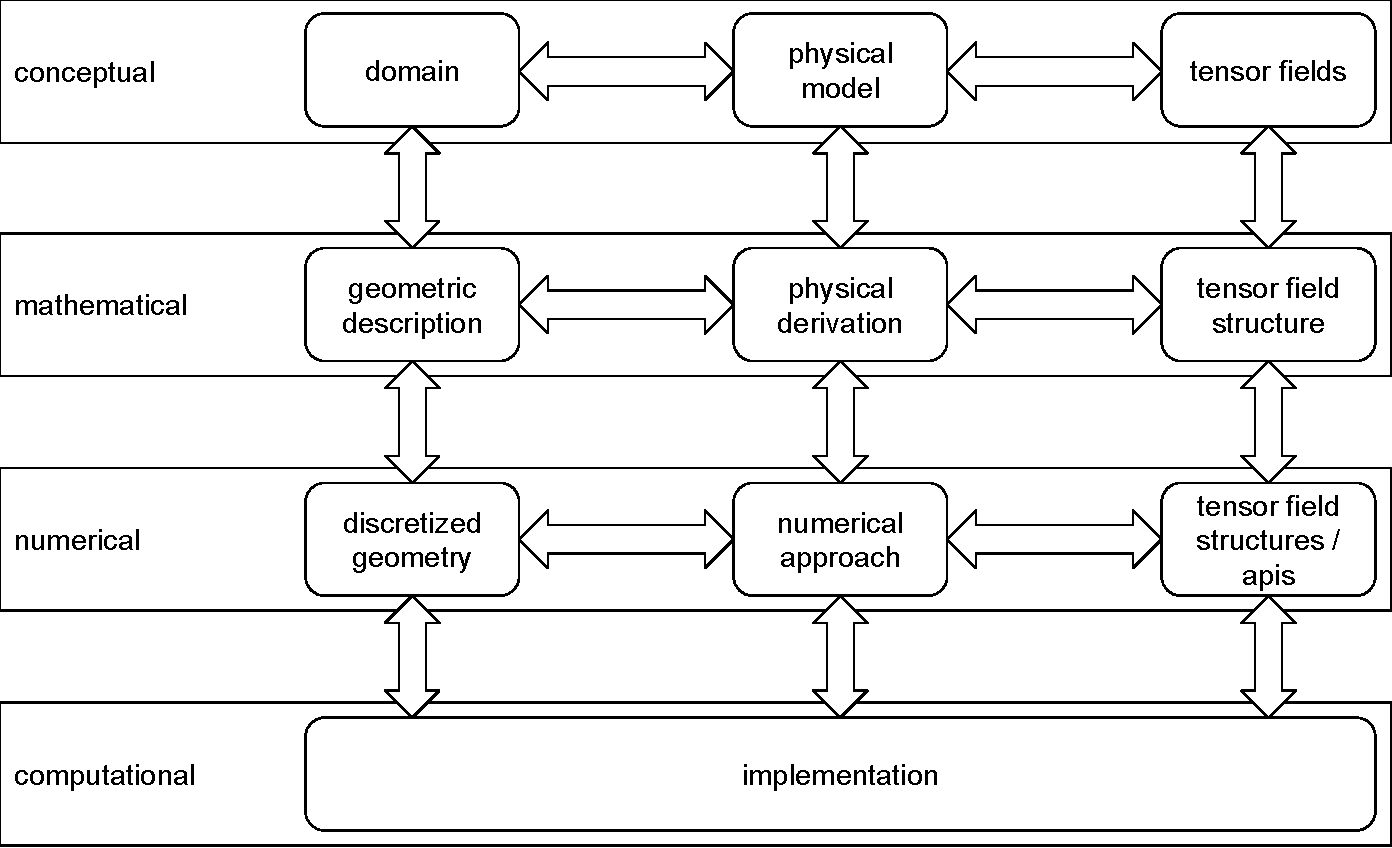
\includegraphics[width=.9\columnwidth]{scale-model-lines}
  \caption{The abstract single-scale model used to inform the development of a multi-scale coupling model.}
  \label{fig:scale-model}
\end{figure}

The Abstract Scale Model (ASM) (illustrated in figure \ref{fig:scale-model}) provides a hierarchical model of the implementation specifics of a single-scale simulation. The model is oriented on the principle of most abstraction to least abstraction along the vertical axis. Each level in the abstraction hierarchy requires information in three different areas: the physics being simulated, the domain (type) over which the simulation is to take place, and the physical tensor fields required to describe the problem.  By specifying or implementing the information required at each node in the ASM a developer will fully describe and produce a single-scale simulation. 

The conceptual physical model is often the starting point in the development of an ASM, as it informs many of the decisions made during the specification of the rest of the model. This high-level description is often specified in terms of the primary physical property(ies) being modeled, e.g. displacements, temperature, trajectories, etc, as well as (typically) one or more conservative laws. The specification of the physical model most directly effects the conceptual domain and conceptual tensor fields. The conceptual domain incorporates both the temporal and spatial domains of the problem, which provides sufficient information to plot the scale on a scale-separation graph. \red{Additionally the conceptual domain includes the specification of e.g. continuum vs. atomistic approaches.} The conceptual tensor fields are directly influenced by the physical model and includes every primary and supporting field required to simulate the physical model as specified by the chosen conservative laws.

\red{add in some references:}
The mathematical physical derivation is a specification of the chosen form of the conservative law(s) from the conceptual physical model and accompanying mathematical requirements. The mathematical geometric description of the domain incorporates the specification of the method of mathematical representation of a domain for the problem, e.g. for a continuum problem a CAD format or grid assumptions. The mathematical tensor field structure for the required fields is specified, including symmetries which allow for tensor order reductions to simplify the mathematical formulations in the physical derivation.

The numerical approach includes the approach to solving the mathematical physical derivation this includes the construction and solution of the discretized model. The discretized geometry specifies the representation of the geometric domain the numerical approach will query and operate on, this includes for instance meshes and grids for continuum problems and discrete particles for MD problems. The tensor field structures and APIs are specified over the discretized geometry and are queried for use in the numerical approach to produce a solution which is also expressed in terms of a tensor field structure. 

The computational implementation of an ASM requires the combination of all numerical specifications in order to produce a final simulation.

\subsection{Abstract Coupling Model}\label{sec:coupling-model}

\begin{figure}
  \centering
  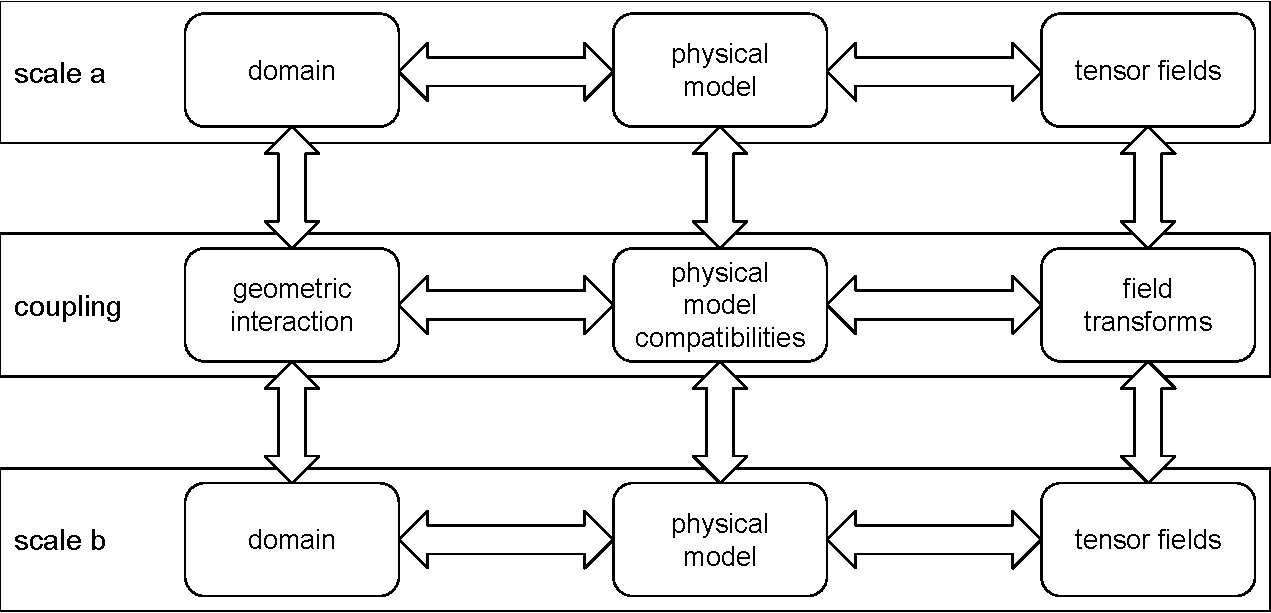
\includegraphics[width=.9\columnwidth]{coupling-model-lines}
  \caption{The abstract multi-scale coupling model used to guide the design of AMSI.}
  \label{fig:coupling-model}
\end{figure}

The ACM is derived from a model initially discussed in \cite{shephard2010component}.

The Abstract Coupling Model (ACM) (seen in figure \ref{fig:coupling-model}) provides a model of the coupling of two distinct realizations of an ASM (fig \ref{fig:scale-model}). The hierarchy of each coupled ASM must be taken into account during the specification of the primary nodes in the ACM. It is convenient to view the ACM as a top-down view of two ASMs and the coupling layer between them. Each of the conceptual, mathematical, and numerical layers must still be considered when specifying nodes in the ACM. Specifying and implementing the ACM fully will result in a valid multi-scale coupling operating between two single-scale simulations.

The physical model compatibility requires the specification of the relationship between the two physical models. This includes any laws relating the physical quantities modeled in the two ASMs, and may require intermediate operations including derived values in order for the two physical models to influence each other. Proceeding down the ASM hierarchy this further requires a particular mathematical derivation, as well as the specification of any numerical operations required to produce all quantities needed to satisfy the mathematical derivation.

The geometric interaction of problem domains includes the specification of each domain on a scale-separation map, as well as the nature of the domain relationship with respect to e.g. overlapping regions/interfaces or full locality of sub-domains for strongly-separated scales. This specifies whether the multi-scale problem is concurrent or hierarchic as discussed in sections \ref{sec:multiscale}. Going down the hierarchy this also includes any mathematical operations required to map spatially between the domains which can include e.g. inverting mappings, interpolation operations, tensor field queries at selected locations. At the numerical level the operations necessitated by the mathematical relationships must be implemented.

The field transforms in a coupling require the specification of all operations required for influences from a field associated with a scale to be incorporated into a field on the other scale(s) in the ACM. At the conceptual level this includes the full set of tensor fields on each scale along with known relevant relationships between the fields. The specification of these operations is primarily mathematical and numerical in nature, and is influence heavily by the physical model compatibility and geometric interactions.

%\red{cite other coupling models?}

\section{AMSI Model Implementation}\label{sec:amsi-mdl-impl}

\section{Parallel Design}\label{sec:amsi-par-design}

\subsection{AMSI Design}\label{sec:amsi-design}

%\cite{belgacem2017future} (this approach is similar to that taken in \cite{} without requiring the inheritence of/restricution to a particular class interface and the addition of a managing process on a single node in the parallel execution space of the simulation)

The AMSI multiscale library provides the facilities to instantiate, manage, and execute dynamic scale coupling operations on otherwise uncoupled single-scale simulation codes. AMSI specifically targets the use-case of a developer taking existing single-scale simulation codes and combining them to produce a new multi-scale code while minimizing intervention in the legacy codebases.

The core of the AMSI multiscale systems operates at the numerical and implementation levels of the ASM and ACM abstraction hierarchy. While developers use a top-down approach to specify and construct a simulation, initial development on AMSI multiscale has focused on providing functionality in a bottom-up fashion. The intent of this approach is to provide a useful set of functionality for developers before working up the abstraction hierarchy to provide facilities for operations required at those levels.

At the lowest-level, the AMSI multiscale library is concerned with the instantiation and management of the individual single-scale codes used in a multi-scale simulation. The parallel structure of HPC machines requires that in order to couple multiple single-scale codes into a multi-scale code, the relationship of those individual single-scale codes to the machine must be modeled by AMSI multiscale. 

The set of threads of execution in a given simulation and their relationship with the physical hardware of the machine is called the parallel execution space (roughly equivalent to MPI\_COMM\_WORLD) of the simulation. AMSI multiscale models the parallel execution space of the whole multi-scale simulation as well as each single-scale code in the multi-scale system, through the use of a Scale.

\subsection{AMSI Scales}\label{sec:scale}

The Scale is a data structure modeling the relationship between the computational level of a single ASM used in the construction of a multi-scale simulation and the parallel execution space of the HPC machine the simulation is executing on. The relationship between the Scale and the parallel execution space is specified by the user using an AMSI multiscale configuration file, further discussed in section \ref{sec:amsi-par-impl}. All Scales present in a multi-scale simulation are instantiated and configured at the beginning of a multi-scale simulation.

Several methods for determining the partitioning of the parallel execution space and assigning the partitions to Scales in a simulation are provided. Scale allocations may be determined by total process count, process ratios between multiple Scales, and additionaly may take advantage of machine introspection operations such as using the \verb-hwloc- \cite{broquedis2010hwloc} hardware locality library in order to take advantage of machine structure for parallel communication operations.

Also during initialization, a main-like function is associated with an individual Scale. A developer may simply reuse the main function of the existing single-scale simulation, however the function is additionally passed an MPI\_COMM associated with the Scale on which parallel operations for the single-scale code modeled by the Scale are to take place.

\subsection{AMSI Couplings}\label{sec:coupling}

The Coupling is a data structure modeling the relationship of units of coupling data between two distinct Scales. The Coupling in AMSI multiscale is not assumed to be symmetric so in order to establish a two-way coupling between Scales a Coupling must be produced for each direction of communication. While it is often the case that a coupling is bi-directional, this is not always the case \cite{gravemeier2008towards}, so this form is preferred. Each Coupling exists on the union of the parallel execution spaces associated with both Scales being coupled, and specifies on Scale as the producer and the other as the consumer.

The Coupling operates at the computational level of the ACM, but is directly informed by specifications at the numerical level. Individual units of scale-coupling data are supplied to the Coupling, e.g. tensor field values located at points as specified by the domain relationship in the ACM. These may be raw values or values derived locally, i.e. the tensor field transformation operations may by applied to the coupling data on either end of the coupling. This allows for minimization of communication overhead whenever possible.

A unit of coupling data generically refers to any data type as the precise implementation or data structure of the data is not assumed by the Coupling or AMSI multiscale until the communication phase of the coupling operation.

The parallel discretization of the numerical domains of the multi-scale problem informs the parallel locality of both the origin and the destination of each unit of scale-coupling data. At present this mapping is taken care of by the developer. Facilitating the automation of the construction of this mapping is the next step in advancing the development of AMSI multiscale up the ASM/ACM abstraction hierarchy.

\section{AMSI Parallel Implementation}\label{sec:amsi-par-impl}

\red{cite the in-progress neuron paper as the most up-to-date reference for biotissue}

Software intended to suppport multi-physics simulations needs to "enable the introduction of new models, algorithms, and data structures" \cite{keyes2013multiphysics}. Further, a set of well-defined modules with distinct interfaces must be implemented, especially as this concerns data ownership and simulation state. State data must be query-able through interfaces in order for coupled codes to maintain consistency throughout the simulation. Further, implementing general code, or providing mechanisms to extract important underlying data in general formats is necessary. This forces multi-physics application developers to adhere to specific data structures and algorithms, or write their own wrapper code in order to translate specialized data structures into more general formats. These issues and rationales for multi-scale software development are further discussed in \cite{keyes2013multiphysics}.

Toward this end AMSI provides a simple API used for multi-scale coupling and scale-sensitive load-balancing operations, and makes no requirement on the application code providing any interfaces for AMSI usage. This allows intervention in legacy code only in locations where multi-scale operations are to be implemented, and where replacement of global collective operations with scale-collective operations is required in order to prevent parallel deadlock. 

%As AMSI is designed around an abstract simulation model, the implementation is not dependent on a particular API or data structure for the discrete domain representation, tensor fields, and numerical implementation of the physical derivation. All computational operations operating on user data are implemented generically to allow the use or arbitrary data types for coupling operations. The user may need to provide a description of the datatype to the underlying parallel communication library for data types requiring a deep copy for serialization. 

\red{Show a multi-scale simulation initialization in AMSI and how construct and execute a Coupling using code snippets.}

\section{Soft-Tissue Implementation}\label{sec:bio-implementation}

Show how AMSI was used with the existing single-scale simulations to construct the biotissue problem.
Discuss the tensor fields involved in the coupling and the transformations required to coupled the physical models together (deformation gradient and stress/stress derivatives), the geometric coupling which is known a-priori due to the strongly-separated nature of this multi-scale simulation since it is hierarchical. 

Discuss the control flow of the single-scale macro and micro simulations. Discuss the modifications to the control flow using AMSI to couple the simulations together into a multi-scale simulation.

Include control flow diagrams for both individual scales as well as the combined multi-scale simulation.

\section{AMSI Performance Measures}\label{sec:amsi-metrics}

Discuss that currently scales must operate on non-overlapping partitions in the parallel execution space, requiring that one scale is idle while the other executes. Address how to minimize this idle time.

What constitutes a good set of results? It likely mostly depends on how we describe our difference from the existing frameworks and what our key goals in AMSI are

  - We mostly focus on the ease of implementing a multi-scale simulation from existing simulations - but this is hard to develop a metric for
  
  - We also want computational efficiency, and while we can calculate our overall compute efficiency for any run we don't really have anything to compare against

\section{Development of Additional Multi-scale Simulations}\label{sec:new-simulations}

\subsection{Hierarchical Simulations}\label{sec:info-passing-examples}

This should be relatively straightforward, just need problem to discuss.

The production of CouplingData objects for hierarchical multi-scale problems is particularly straightforward as the domain relationship is well-established a-priori. 

\subsection{Coupled-Domain Simulations}\label{sec:concurrent-examples}

Discussion of obstacles being worked on towards concurrent multi-scale with discussion of at least one particular problem.

The production of a CouplingData object derived from the relationship between the domains in a concurrent partitioned-domain problem is a complex operation currently undergoing development. 


\bibliographystyle{siamplain}
\bibliography{multiscale_theory,multiscale_frameworks,software}
\end{document}
